%\setcounter{section}{0}
%\setcounter{subsection}{0}
%\setcounter{subsubsection}{0}
%\setcounter{equation}{0}
%\pagenumbering{arabic} 
%\setcounter{page}{0}    %%%%%KKD used \setcounter{page}{0}  
%\oddsidemargin 0.9 cm 
%\evensidemargin -.4 cm
%\setlength{\textwidth}{152.4 mm}
\chapter{Search for Pair Production of First Generation Leptoquarks  \label{Search for pair Production of First Generation Lepto Quarks}}


Leptoquark pair-production at the LHC of CERN proceeds primarily through gluon-gluon fusion, with a smaller contribution from quark-antiquark annihilation.
Here, the leptoquark mass (M$_{LQ}$) and the Yukawa coupling $\lambda$ to leptons and quarks are relevant production and decay parameters.
The production cross section is nearly independent of $\lambda$.

A leptoquark will decay into a lepton and a quark, giving rise to a final state containing high-momentum leptons and jets.
The decay into a charged lepton and a quark has branching fraction $\beta$, while the decay into a neutrino and a quark has branching fraction $1-\beta$, ( $\beta$ is a free parameter). Previous searches for rare processes mediated by lepton number violation, and flavor-changing neutral currents prefer leptoquarks at LHC-accessible mass ranges which couple to leptons and quarks of
  the same generation %(no mixing)~\cite{Buchmuller,FCNC}. 
The first generation leptoquarks, we assume leptoquarks decay to electrons and electron neutrinos, leading to following three final states:
\begin{itemize}
  \item Two electrons and two jets: each leptoquark decays into an electron and a quark;
  \item One electron, MET, and two jets: one leptoquark decays into an electron and a quark, while the other decays into a neutrino and a quark; and 
  \item No electrons, MET, and two jets: each leptoquark decays into a neutrino and a quark.
\end{itemize}
The final state branching fractions are $\beta^2$, $2\times\beta(1-\beta)$, and $(1-\beta)^2$, respectively.
We consider two values of $\beta$: 1, which corresponds to leptoquarks always decaying to the first final state; and 0.5,
where 50\% of leptoquarks decay to the second final state, with 25\% decaying to the first and 25\% decaying to the third final states.
The first and second final states are denoted as $eejj$ and $e{\nu}jj$.
In this analysis, we search for leptoquark decays in the first final state only, $eejj$.

Previous searches have not detected any leptoquarks. Recently, CMS recently published a search ~\cite{CMS-PAS-EXO-12-041} using about 20~$\text{fb}^{-1}$ of 2012 LHC data recorded at $\sqrt{s}=8$~TeV, which gave first generation
leptoquark mass limits of less than 1010 (850) GeV for $\beta=1$($0.5$).%~\cite{exo-12-041-paper}.
 Similarly, ATLAS used the 2012 LHC data to set first generation leptoquark mass limits of less than 1050 (900) GeV for $\beta=1$($0.5$),
and also looked at the possibility of $\beta=0.2$, which gave a mass limit of 900 GeV~\cite{atlasLQ8TeVpaper}.
All of the above limits are set at the 95\% CL.



\section{Event Selection}


The $eejj$ final state is the result of two pair-produced leptoquarks each decaying to an electron and a jet, where the branching fraction $\beta$ as defined previously is equal to 1. Events containing at least two electrons and two jets are selected, where the two leading $\rm p_{T}$ electrons and jets are used in the analysis.

\subsubsection{Preselection}
\label{subsubsec:eejjPreselection}
The preselection is aimed at selecting background-dominated event sample in order to compare MC simulated background predictions with the data.
The corresponding selection criteria that the candidate event should
\begin{itemize}
  \item Passes the signal trigger. The signal trigger has the following criteria
    \begin{itemize}
     \item Single electron with online $\rm p_{T}$ greater than 27 GeV,
     \item the electron has to satisfy loose idenitication criteria (loose means , loose compared to the offline HEEP criteria which will be defined, later), and 
     \item the techical CMS jargon is: \texttt{HLT\textunderscore Ele27\textunderscore WPLoose\textunderscore Gsf\textunderscore v*},

     \end{itemize}

  \item Contains exactly two electrons passing HEEP (High Energy Electrons) ID~\ref{fig:HEEPID6p0}, additionally having ECAL supercluster ${E_T} >$ 50 GeV and ECAL supercluster pseudorapidity $|\eta_{SC}| <$ 2.5 (HEEP selection criteria gives high efficiency for high energy electrons),
  \item Contains no muons, where muons are selected with $p_T >$ 45 GeV and $|\eta| <$ 2.1,
  \item Contains at least two jets with $p_T >$ 50 GeV and $|\eta| <$ 2.4,
  \item Have $m_{ee} >$ 50 GeV, where $m_{ee}$ is the dielectron invariant mass, and 
  \item Have $S_T >$ 300 GeV, where $S_T$ is the scalar sum of  $p_T$ of the two electrons and the two leading jets.
  
\end{itemize}
After applying these criteria, the overall MC background agreement with the data is examined in a series of plots, they show a quite good agreement of the data with the SM backgrounds. The data-MC agreement in terms of above last two variables could be seen in Fig.~\ref{figure:DatavsBkgPreselection}. The ratio plots have been provided for a better view of the data-MC agreement.

\begin{figure}[h]
\centering
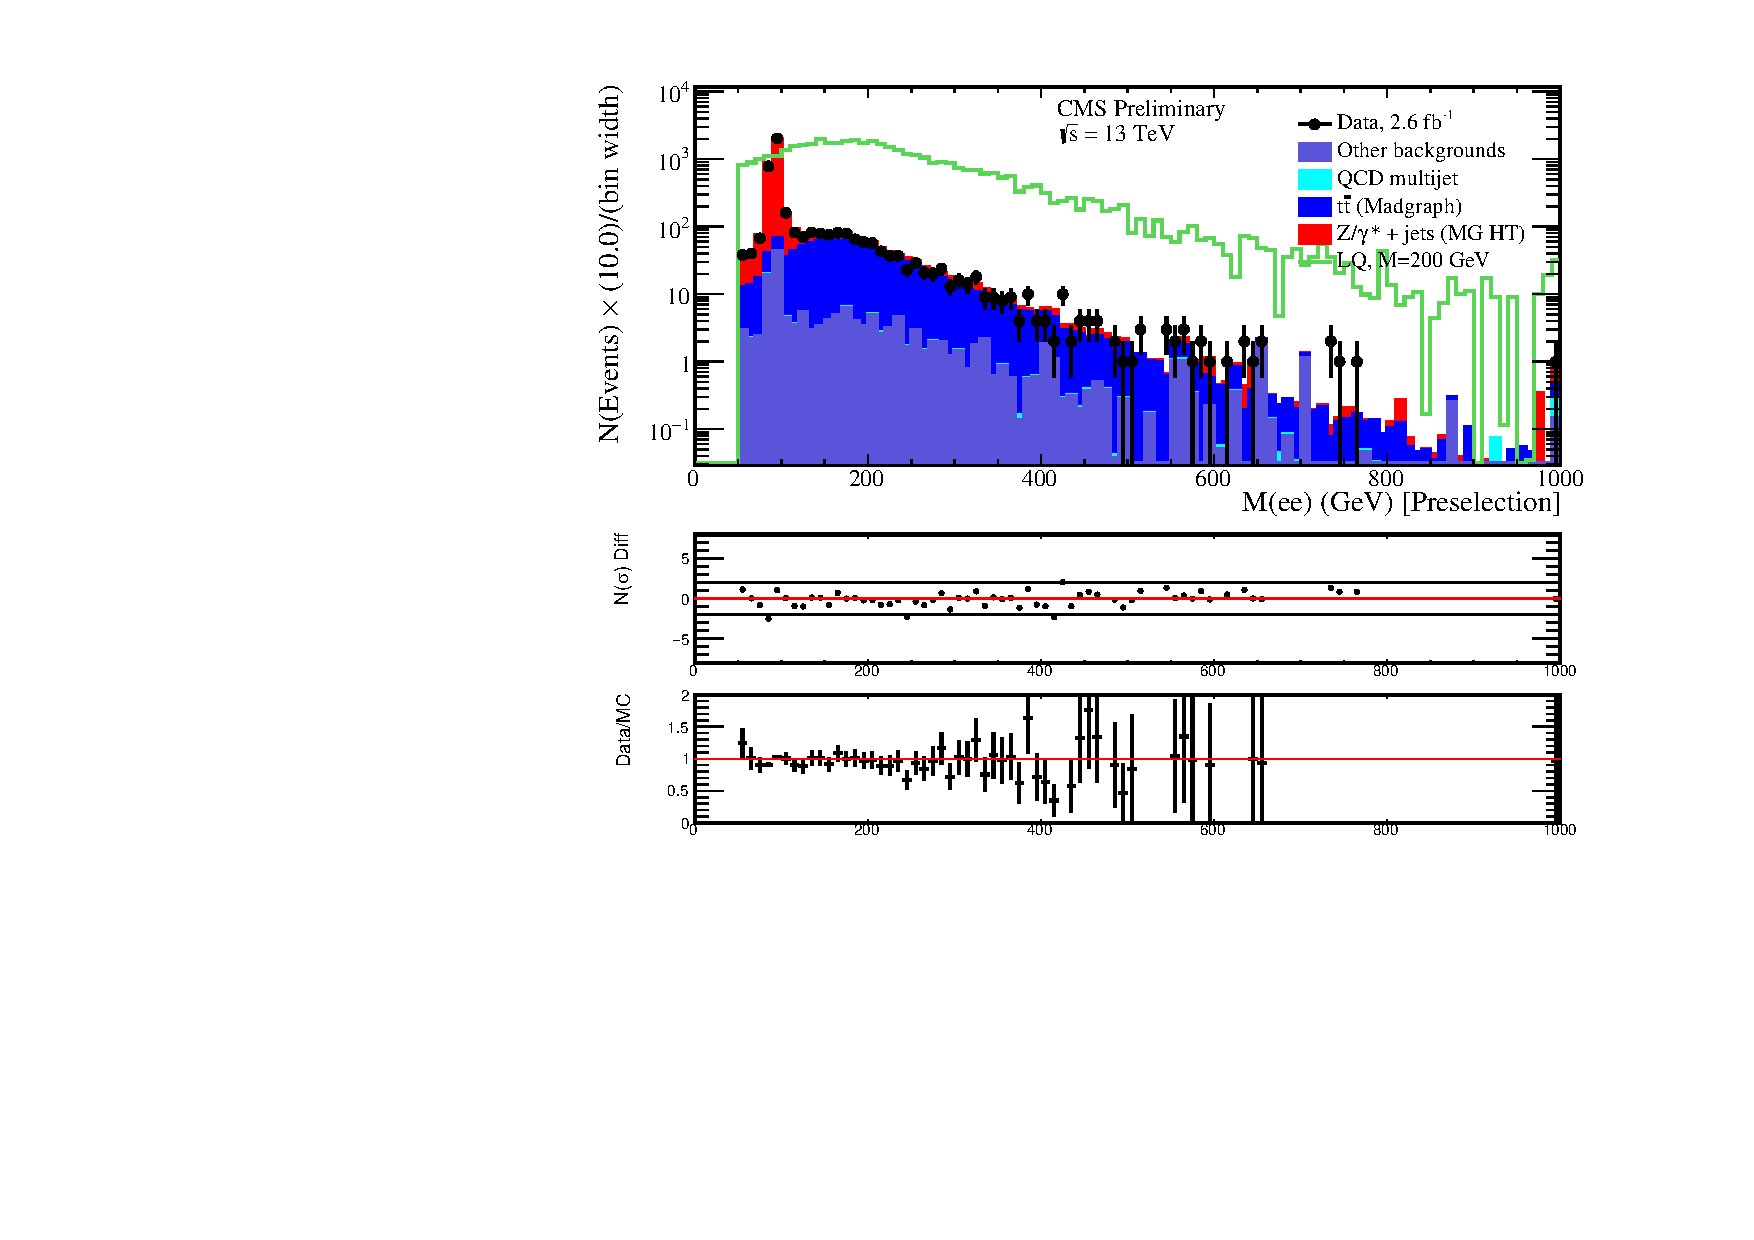
\includegraphics[width=0.32\textwidth]{/home/bibhu/Desktop/PhDThesis/PhDThesis/chapter7/Mee_PAS_eejj.pdf}
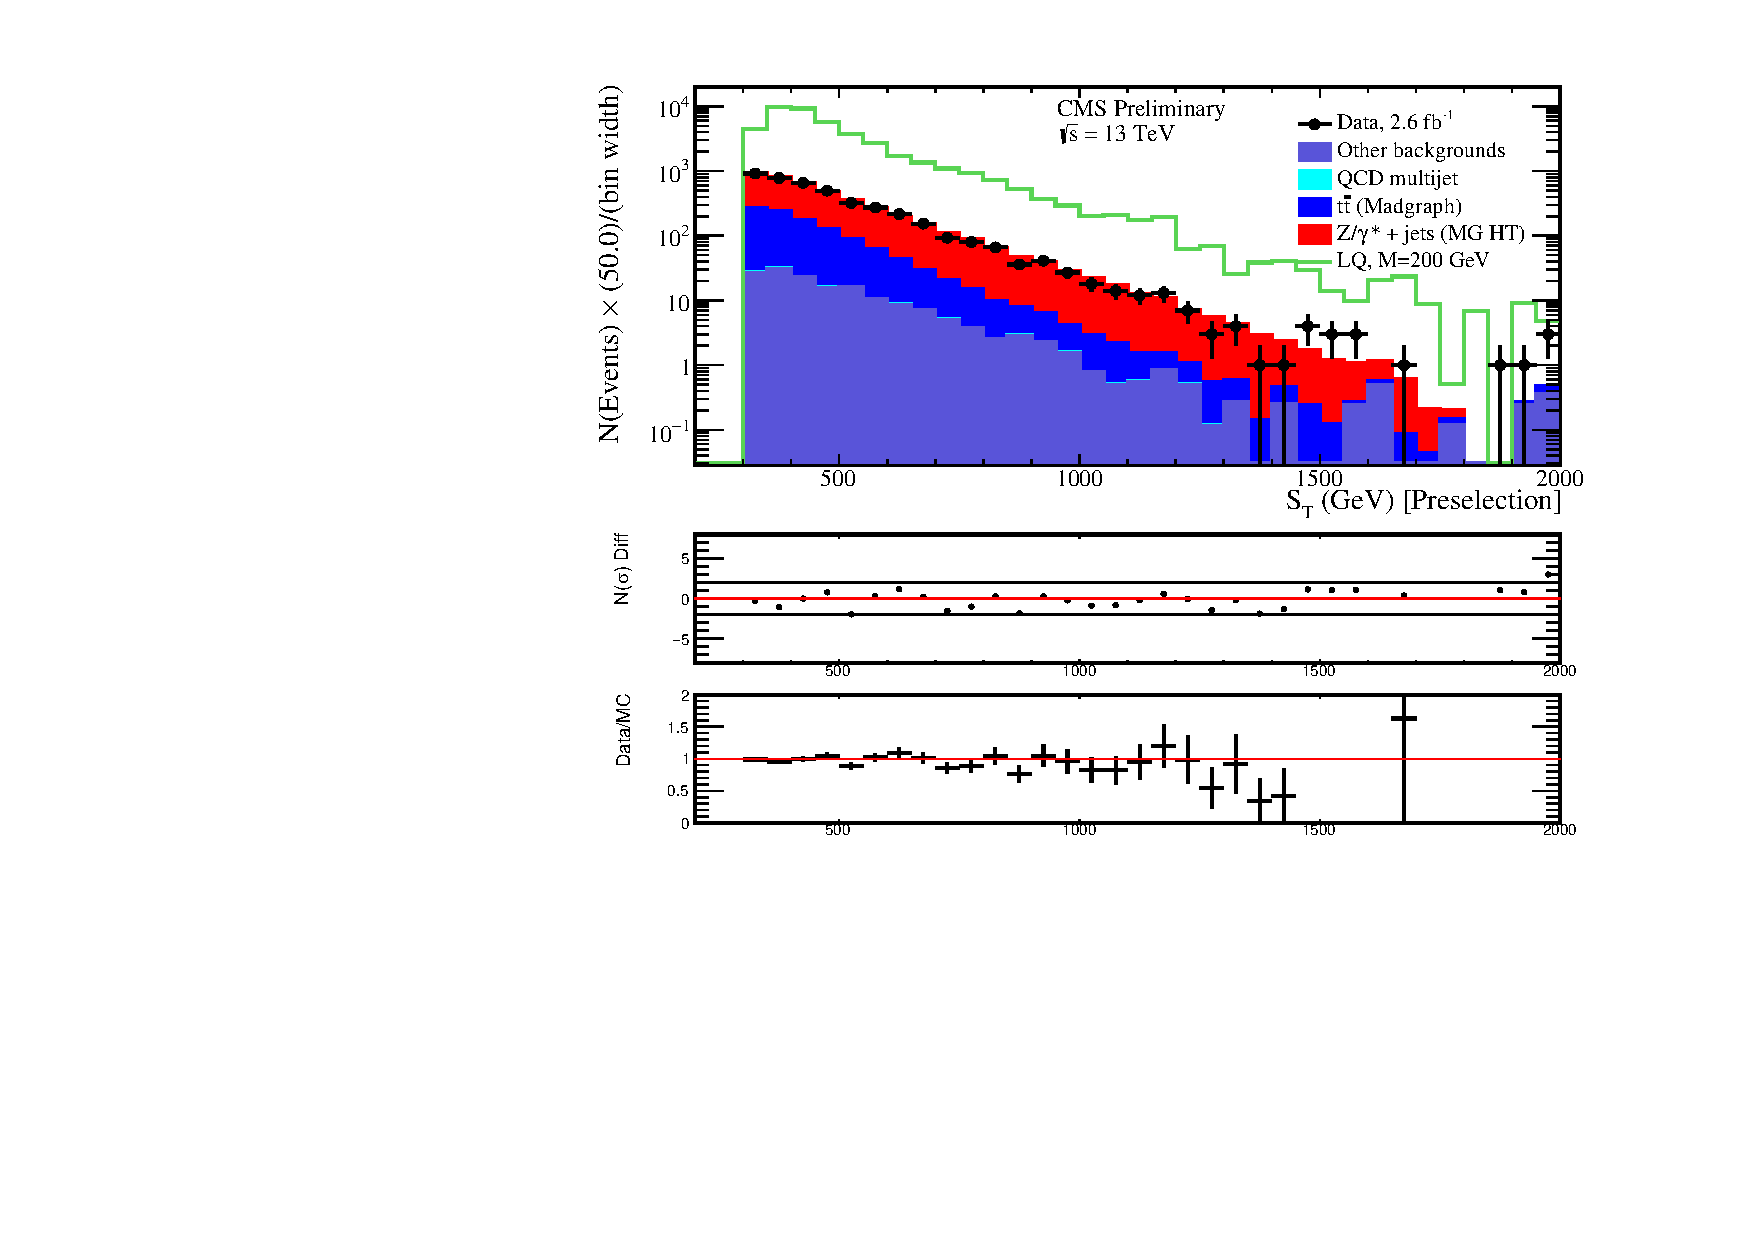
\includegraphics[width=0.32\textwidth]{/home/bibhu/Desktop/PhDThesis/PhDThesis/chapter7/sT_PAS_eejj.pdf}
\caption{\label{figure:DatavsBkgPreselection}Data vs. background plots for$\rm M_{ee}$(left) and $\rm S_{T}$(right) after Preselection}
\end{figure}



\begin{figure}[h]
\begin{center}
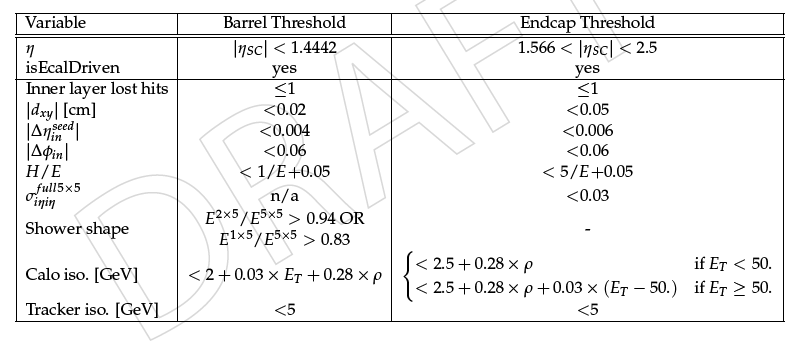
\includegraphics[height=7cm, width=15cm]{/home/bibhu/Desktop/PhDThesis/PhDThesis/chapter7/HEEPID6p0.png}

\caption{\label{fig:HEEPID6p0} HEEP Identification electron selection criteria used for the analysis.}
\end{center}
\end{figure}



\newpage
\subsubsection{final selection}
In order to maximize the presence of signal and reduce the background, we have optimized the set of cuts on three variables . They are 
\begin{itemize}
 \item $M_{LQ}$,
 \item  $m_{ee}$ and
 \item  $m_{ej}^{min}$. As each leptoquark decays to an electron and a quark, when we choose the correct $e$ and $j$ pair, mass difference from the two reconstructed LQs should be very small. So out of 2 electrons and 2 jets we make four combinations to see which combinations gives minimum difference between the $m_{e,j}$ mass. We again use this variable to optimize the sensitivity.
\end{itemize}

The variables $S_T$, $m_{ee}$, and $m_{ej}$ are varied independently over a range of values, and the thresholds which maximize the optimization metric are obtained for each leptoquark mass point. The optimization metric considered is called `Punzi's Significance~\cite{PunziSignificance} in Eq.~\ref{eq:punziOpt}, where t represents an attempted set of cuts, $\epsilon(t)$ is the efficiency times acceptance of the signal, a is the one-sided significance required in standard deviations, and B(t) is the expected number of background events. We choose a = 5 to require 5$\sigma$ discovery significance. A unique property of the Punzi criterion is that is does not depend on the signal cross section, but only on its acceptance times efficiency. 

%\begin{linenomath}
  \begin{equation}
    \frac{\epsilon(t)}{a/2+\sqrt{B(t)}}
    \label{eq:punziOpt}
  \end{equation}
%\end{linenomath}

The optimized set of cuts are shown in the Table ~\ref{tab:optimizedThresholds}.
\begin{table}[h]
  \begin{center}
    %\tiny
    \caption{Optimized final selection thresholds for the $eejj$ analysis.}
    \label{tab:optimizedThresholds}
    \begin{tabular}{|c||c|c|c|}\hline
      $M_{LQ}$ [GeV]     &     $S_T$ [GeV] $ >$       &      $m_{ee}$ [GeV] $ >$     &     $m_{ej}^{min}$ [GeV] $ >$ \\ \hline\hline
      200 & 340 & 130 & 160 \\ 
      \hline 
      250 & 405 & 140 & 205 \\ 
      \hline 
      300 & 470 & 155 & 245 \\ 
      \hline 
      350 & 535 & 165 & 285 \\ 
      \hline 
      400 & 595 & 175 & 325 \\ 
      \hline 
      450 & 660 & 185 & 360 \\ 
      \hline 
      500 & 720 & 195 & 400 \\ 
      \hline 
      550 & 780 & 205 & 435 \\ 
      \hline 
      600 & 840 & 210 & 470 \\ 
      \hline 
      650 & 900 & 220 & 500 \\ 
      \hline 
      700 & 960 & 230 & 535 \\ 
      \hline 
      750 & 1015 & 235 & 565 \\ 
      \hline 
      800 & 1075 & 245 & 595 \\ 
      \hline 
      850 & 1130 & 250 & 625 \\ 
      \hline 
      900 & 1190 & 255 & 650 \\ 
      \hline 
      950 & 1245 & 265 & 675 \\ 
      \hline 
      1000 & 1300 & 270 & 705 \\ 
      \hline 
      1050 & 1355 & 275 & 725 \\ 
      \hline 
      1100 & 1410 & 280 & 750 \\ 
      \hline 
      1150 & 1460 & 285 & 775 \\ 
      \hline 
      1200 & 1515 & 285 & 795 \\ 
      \hline 
      1250 & 1565 & 290 & 815 \\ 
      \hline 
      1300 & 1615 & 295 & 830 \\ 
      \hline 
      1350 & 1670 & 300 & 850 \\ 
      \hline 
      1400 & 1720 & 300 & 865 \\ 
      \hline 
      1450 & 1770 & 300 & 880 \\ 
      \hline 
      $\geq$1500 & 1815 & 305 & 895 \\ 
      \hline 
    \end{tabular}

\end{center}
\end{table}


\section{ Backgrounds}

The major backgrounds from SM processes are $Z+$jets and $t\bar{t}$, whereas single top, $W+$jets, diboson, and $\gamma$+jets contribute at a lower level. There is also an instrumental background from QCD multijet events with jets faking as electrons and passing the HEEP ID. Below we describe briefly about the estimation of QCD background as this is the part where we contribute maximally. QCD contribution to the signal region is small compared to the $Z+$jets and $t\bar{t}$ but as QCD is one the less understood process, so a careful attention is needed to estimate background. We eployed a fully data driven background estimation method for QD estimation.

\subsection{QCD multijet :}
QCD events enters our signal region because of misidentification of jets are electrons. So our HEEP criteria has finite fake rate (FR). Here we define the fake rate as the probability of a jet to be misidentified as electron. Mathematically,

  \begin{equation}
    Fake Rate = \frac{N_{pass,HEEP,jets}}{N_{total,jets}}
    \label{eq:FakeRate}
  \end{equation}

As our signal region has a requirement of two electrons, we take a control sample of two electrons with very loose criteria imposed on them. This control sample becomes a jet dominated region. Then we estimate the number of QCD events that contribute to the signal region 

   \begin{equation}
    N_{QCD}^{eejj} = \sum_{events} FR_{1}\otimes FR_{2}
    \label{eq:FakeRate}
  \end{equation}

where $FR_{1}$ and $FR_{2}$ are the fake rates of the two electrons. The fake rates are determined in a data driven way decribed in detail in the ~\cite{CMS-PAS-EXO-16-043}.


\section{Results and Statistical Interpretation}

Similar to the two SUSY analyses~\cite{CMS-PAS-SUS-15-002,CMS-PAS-SUS-16-014}, we observe no significant excess of events as compared to the SM backgrounds. A broad excess of the events that was seen in the 8 TeV analysis~\cite{CMS-PAS-EXO-12-041} has dissapeared with the 2015 data. The data-MC agreement after the final selection for the LQ mass point 650 could be seen from Fig.~\ref{figure:DataMCfinalSelection}. We set the upper limits on the cross section times branching fraction using the LHC style approach. Fig. ~\ref{figure:LimitLQ12016} shows both the observed and expected limits for different leptoquark masses. We exclude leptoquark masses up to 1130 GeV from this study. 

\begin{figure}[h]
\centering
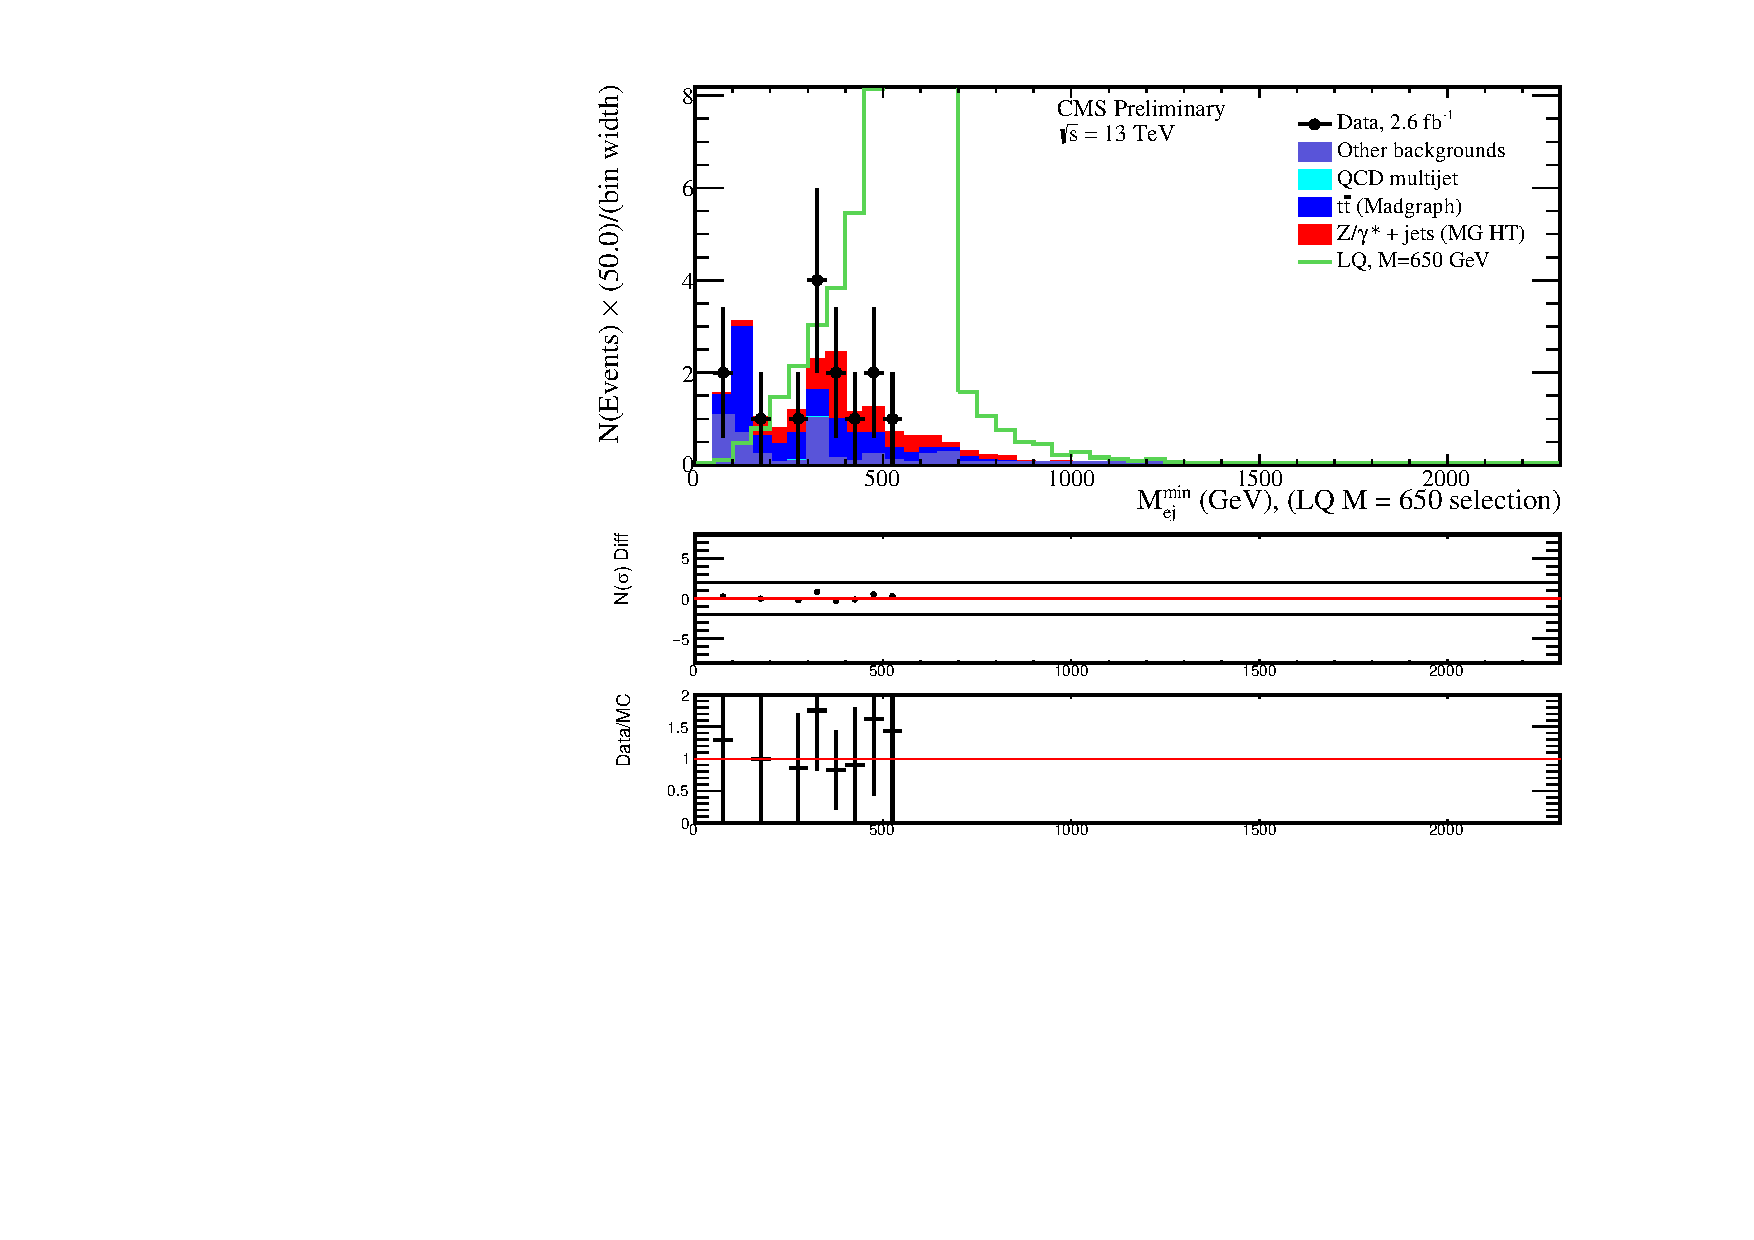
\includegraphics[width=0.32\textwidth]{/home/bibhu/Desktop/PhDThesis/PhDThesis/chapter7/Mej_selected_min_nMinus1_LQ650_eejj.pdf}
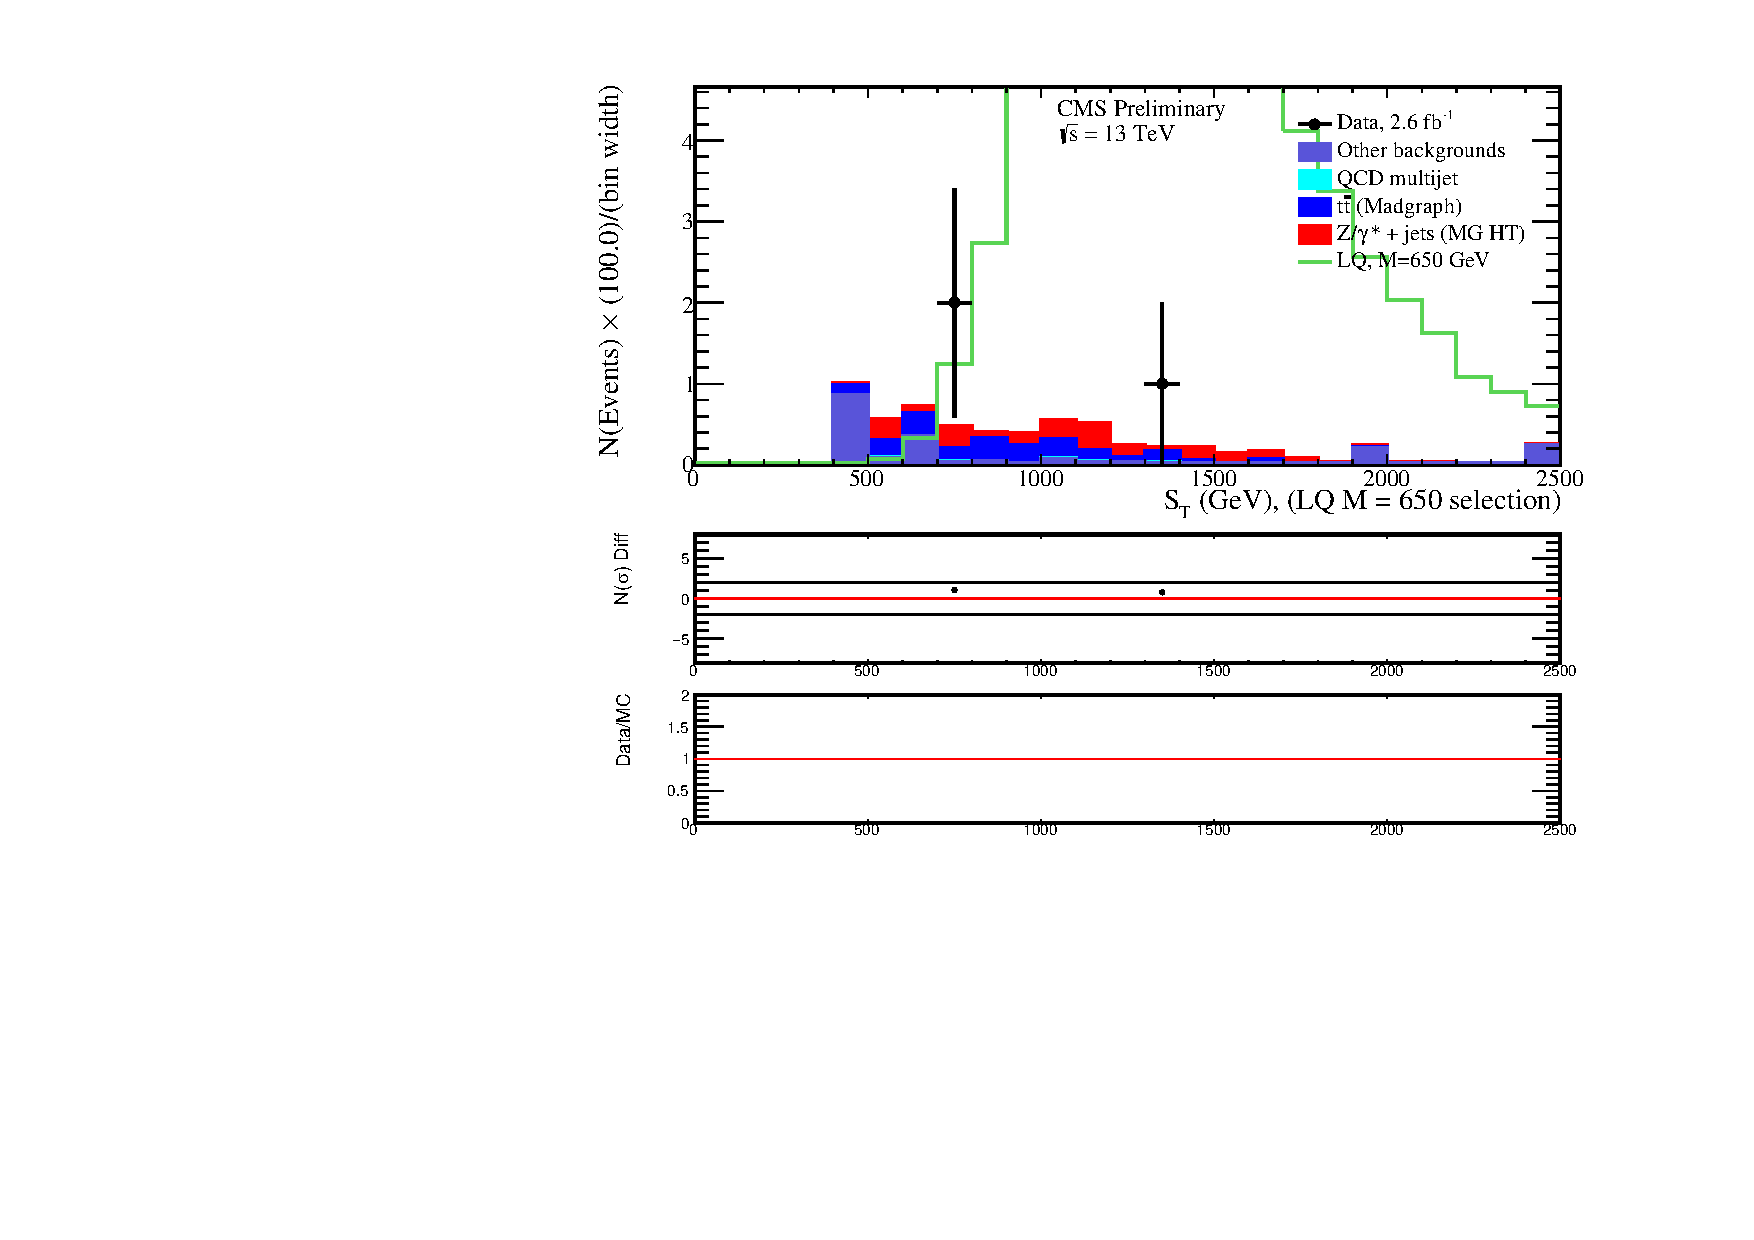
\includegraphics[width=0.32\textwidth]{/home/bibhu/Desktop/PhDThesis/PhDThesis/chapter7/sT_eejj_nMinus1_LQ650_eejj.pdf}

\caption{\label{figure:DataMCfinalSelection} The data vs. MC for LQ mass point 650 GeV in $M_{ej}$ (left) and $S_{T}$ (right). }
\end{figure}



\begin{figure}[h]
\centering
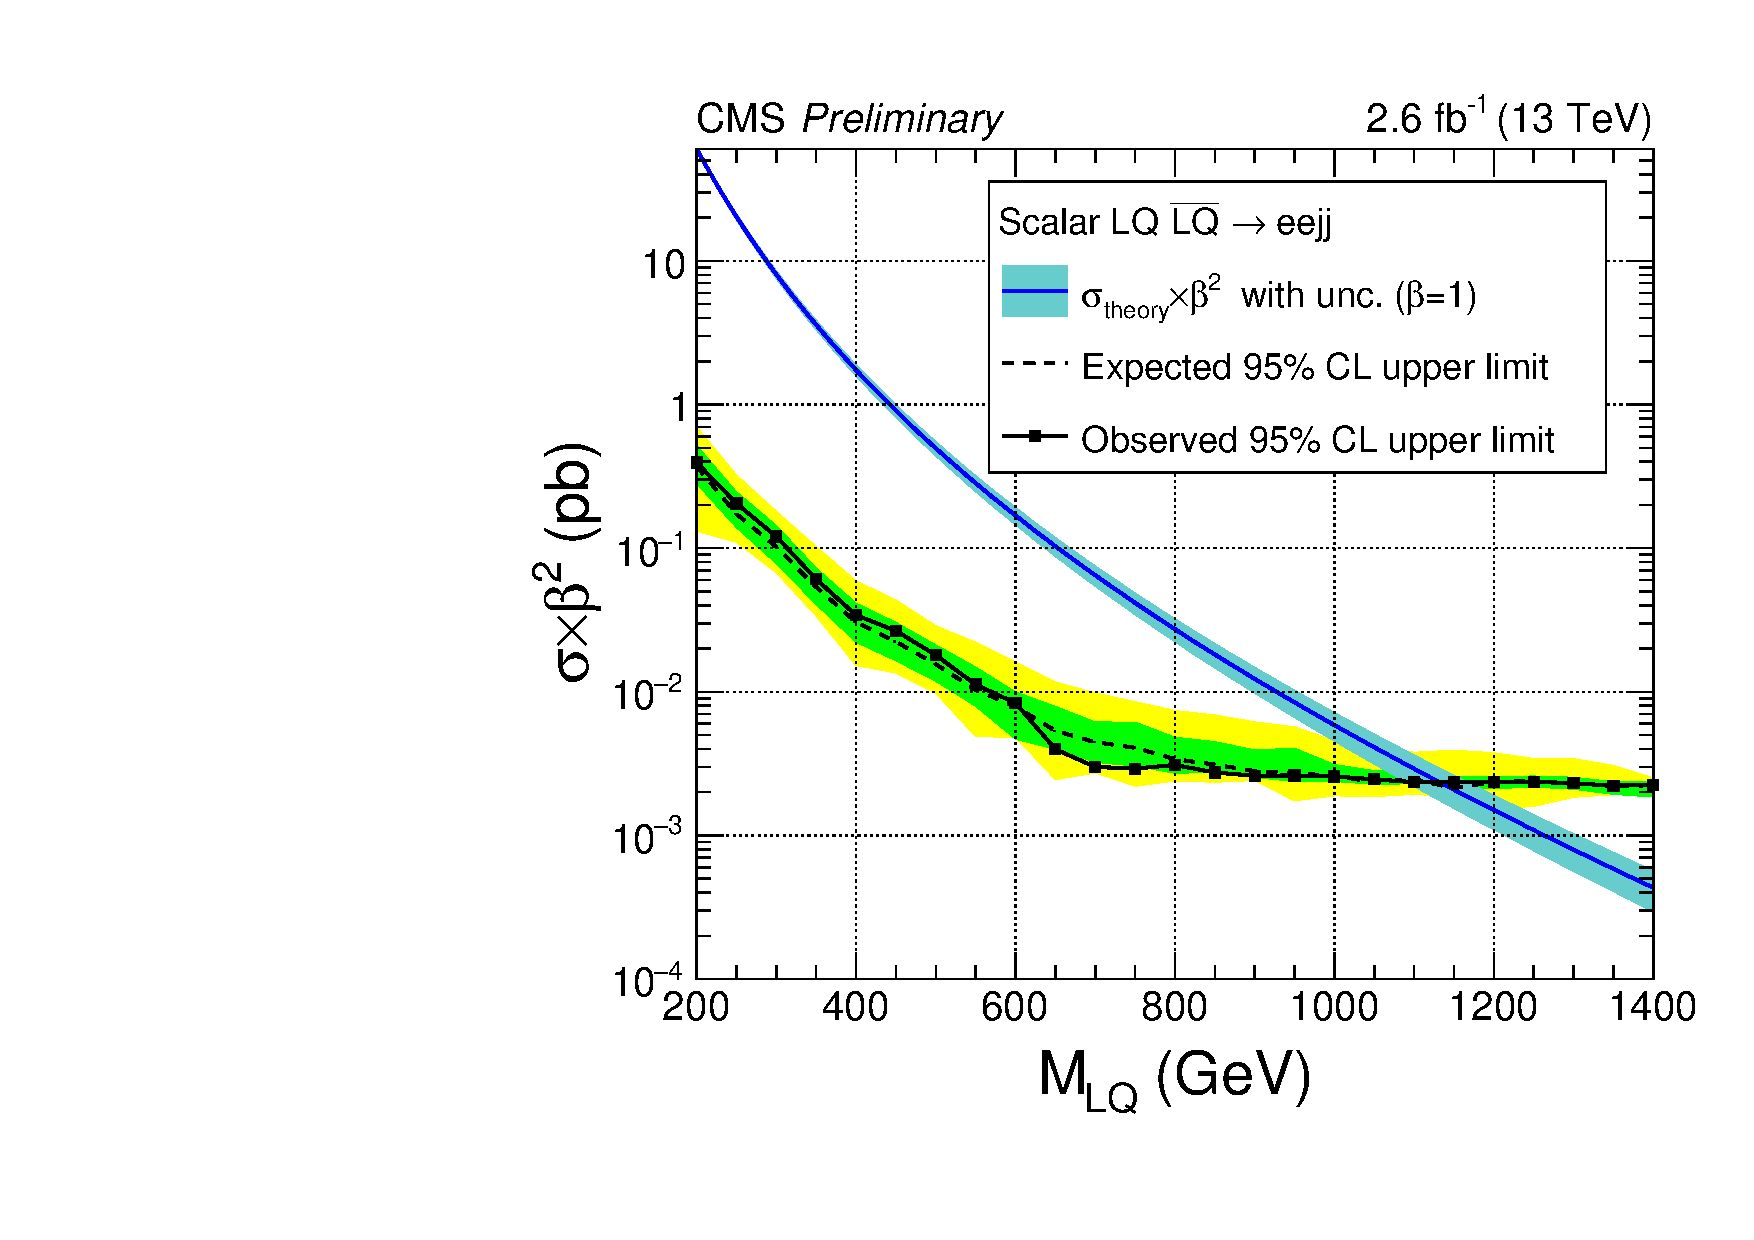
\includegraphics[width=0.32\textwidth]{/home/bibhu/Desktop/PhDThesis/PhDThesis/chapter7/LQLimitPlot.pdf}
\caption{\label{figure:LimitLQ12016}The 95\% CL upper limits on the production cross sections as a function of the leptoquark mass.}
\end{figure}











